\documentclass[11pt,a4paper]{article}
\usepackage[margin=0.85in]{geometry}
\usepackage{graphicx}
\usepackage{amsmath}
\usepackage{amssymb}
\usepackage{booktabs}
\usepackage{hyperref}
\usepackage{float}
\usepackage{caption}
\usepackage{subcaption}
\usepackage{listings}
\usepackage{xcolor}
\usepackage{titlesec}
\usepackage{enumitem}
\usepackage{tabularx}
\usepackage{fancyhdr}
\usepackage{microtype}

% Compact paragraph and list spacing
\setlength{\parskip}{4pt plus 1pt minus 1pt}
\setlength{\parindent}{0pt}
\setlist{topsep=2pt, partopsep=0pt, parsep=1pt, itemsep=2pt}

% Compact section titles
\titlespacing*{\section}{0pt}{10pt plus 2pt minus 2pt}{4pt plus 1pt minus 1pt}
\titlespacing*{\subsection}{0pt}{8pt plus 2pt minus 1pt}{3pt plus 1pt minus 1pt}
\titlespacing*{\subsubsection}{0pt}{6pt plus 1pt minus 1pt}{2pt plus 1pt minus 1pt}

% Float and caption spacing optimization
\setlength{\floatsep}{6pt plus 2pt minus 2pt}
\setlength{\textfloatsep}{8pt plus 2pt minus 2pt}
\setlength{\intextsep}{6pt plus 2pt minus 2pt}
\captionsetup{font=small,labelfont=bf,skip=4pt}

\pagestyle{fancy}
\fancyhf{}
\rhead{\footnotesize DAC-301 Deep Learning Assignment}
\lhead{\footnotesize Ankur Dahiya}
\rfoot{\footnotesize Page \thepage}
\renewcommand{\headrulewidth}{0.4pt}

\definecolor{codegray}{rgb}{0.96,0.96,0.96}
\definecolor{codeblue}{rgb}{0.0,0.3,0.7}
\definecolor{codegreen}{rgb}{0.1,0.5,0.1}

\lstset{
  language=Python,
  backgroundcolor=\color{codegray},
  basicstyle=\ttfamily\scriptsize,
  keywordstyle=\color{codeblue}\bfseries,
  commentstyle=\color{codegreen}\itshape,
  breaklines=true,
  frame=single,
  framerule=0.4pt,
  rulecolor=\color{black!20},
  captionpos=b,
  xleftmargin=1em,
  framexleftmargin=1em,
  aboveskip=4pt,
  belowskip=4pt
}

\hypersetup{
  colorlinks=true,
  linkcolor=blue!70!black,
  urlcolor=blue!70!black,
  citecolor=blue!70!black
}

\title{
  \vspace{-1.2cm}
  \textbf{\Large DAC-301: Deep Learning Assignment}\\[0.3em]
  \large Glasses Classification using a Custom Convolutional Neural Network\\[0.2em]
  \normalsize Kaggle Competition Report
}
\author{\textbf{Ankur Dahiya}}
\date{October 2026}

\begin{document}

\maketitle
\vspace{-0.6cm}
\begin{abstract}
\noindent In this assignment, we design, implement, and evaluate a high-performing Convolutional Neural Network (CNN) from scratch in PyTorch to classify whether a person in a facial image wears glasses. Adhering strictly to course constraints (no pre-trained backbones, no transfer learning, pure PyTorch operations without NumPy in the network, and exclusion of ViTs/DDPMs), our optimal 5-stage VGG-style architecture coupled with high-resolution $224\times 224$ inputs, stochastic augmentations, AdamW optimization with Cosine Annealing, and Test-Time Augmentation (TTA) achieved a \textbf{Public Leaderboard score of 0.99872 (1st Place)}.
\end{abstract}
\vspace{-0.2cm}

\section{Introduction and Task Overview}
The objective of this assignment is to build a binary classifier to predict whether an individual wears glasses from facial images. The dataset comprises $\sim$25k labeled training images and 5,412 unlabelled test images. Final predictions must be submitted as a \texttt{submission.csv} matching Kaggle requirements.

\textbf{Competition Guidelines Summary:}
\begin{itemize}
  \item \textbf{Individual Work:} Single submission per participant; codebase and notebook must accompany predictions.
  \item \textbf{Framework Constraint:} Strictly implemented using PyTorch. The use of NumPy within the network implementation and forward/loss pipeline is prohibited.
  \item \textbf{No Transfer Learning:} Models must be initialized with random weights and trained strictly from scratch.
  \item \textbf{Architecture Scope:} Traditional neural networks and convolutional networks (CNNs) taught in class are permitted. Advanced generative/attention models like ViTs and DDPMs are restricted.
  \item \textbf{Hyperparameter Interface:} Must allow tuning of \texttt{lr}, \texttt{momentum}, \texttt{num\_hidden}, \texttt{sizes}, \texttt{activation}, \texttt{loss}, \texttt{opt}, \texttt{batch\_size}, and \texttt{anneal}.
\end{itemize}

\section{Exploratory Data Analysis (EDA)}
We performed exploratory analysis on the 24,499 training images (\texttt{train.csv}) to characterize class balance, frame types, and pixel distributions.

\begin{figure}[H]
  \centering
  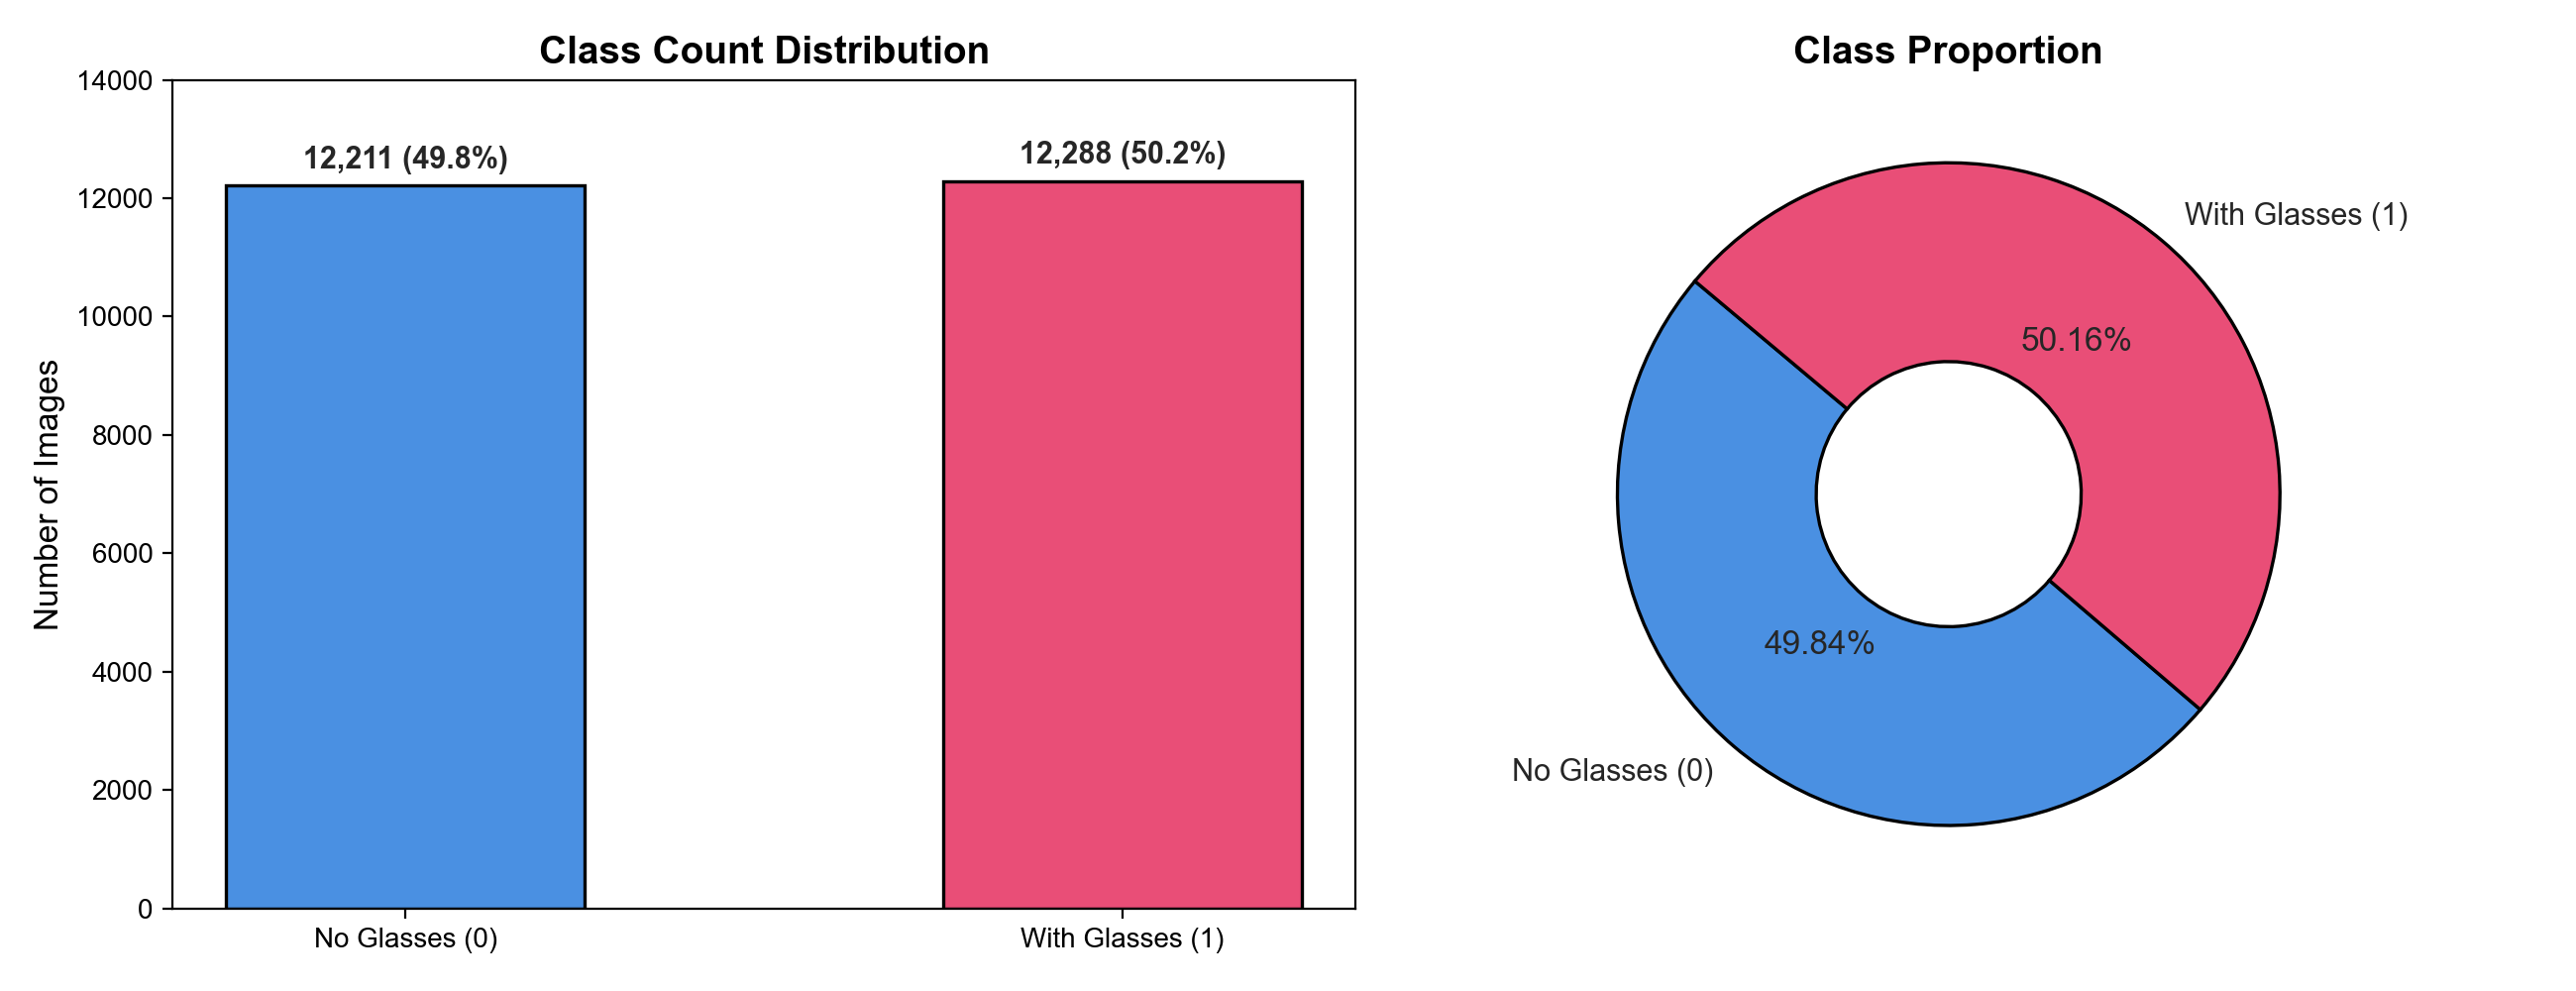
\includegraphics[width=0.78\textwidth]{eda_class_distribution.png}
  \caption{Class balance of the training dataset. Left: Sample count. Right: Proportions.}
  \label{fig:class_dist}
\end{figure}

The distribution is remarkably balanced: \textbf{12,211 images (49.84\%)} without glasses and \textbf{12,288 images (50.16\%)} with glasses. Consequently, standard cross-entropy loss without class re-weighting or focal loss is statistically optimal.

\begin{figure}[H]
  \centering
  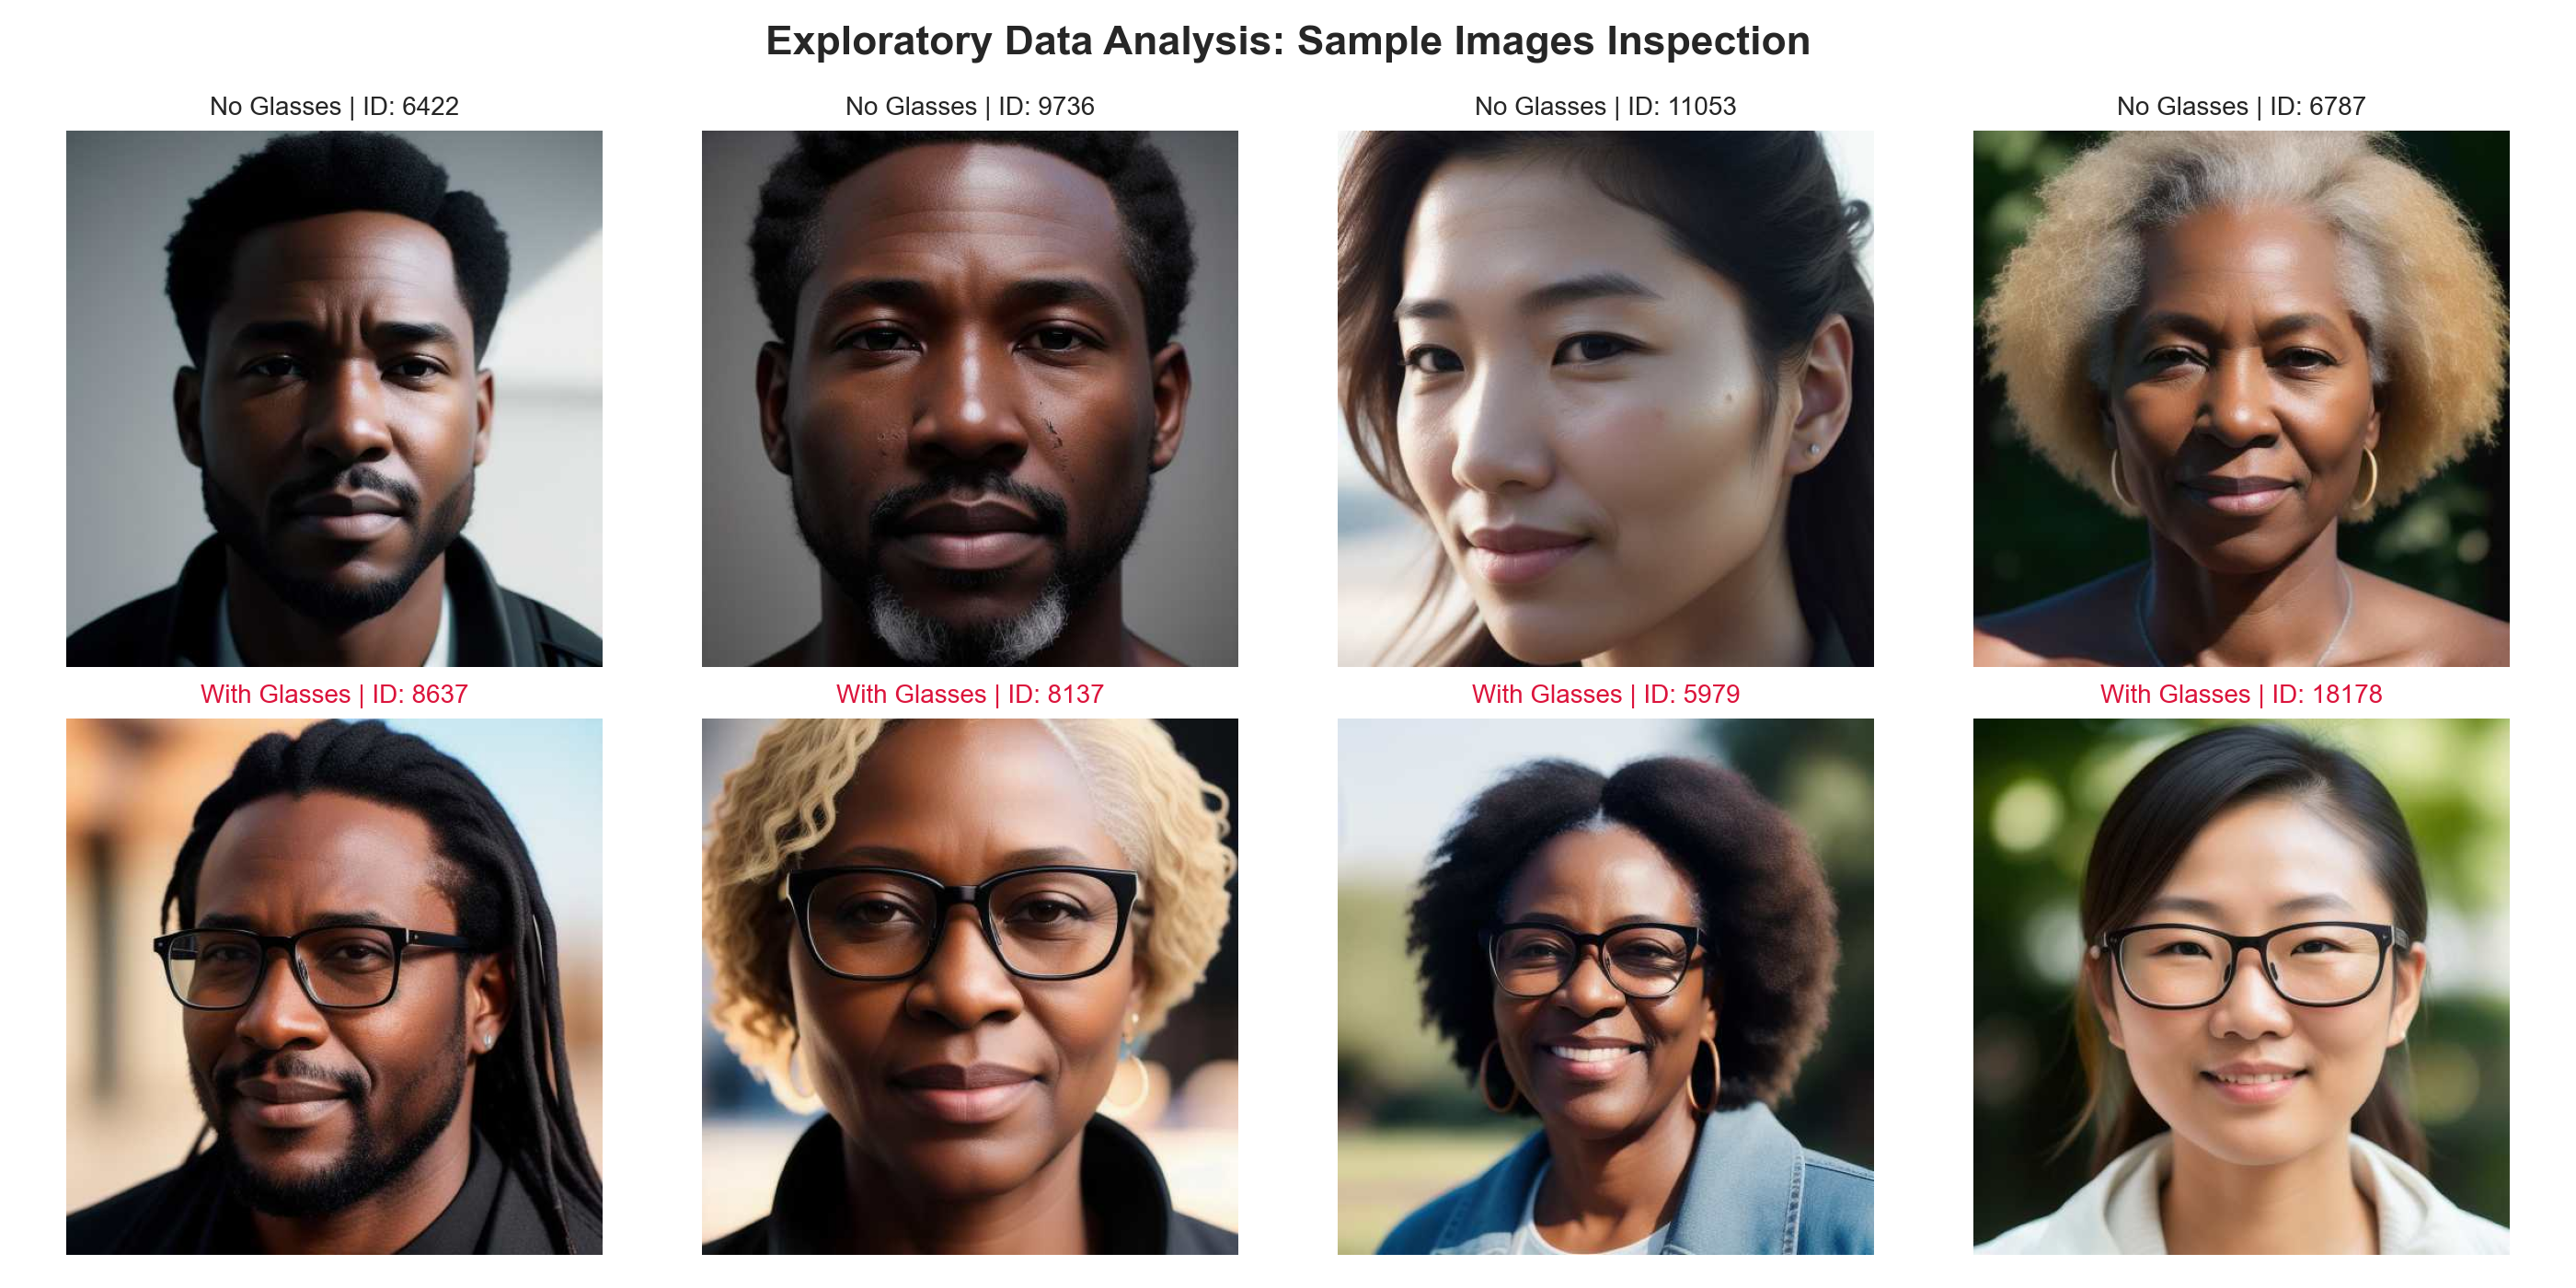
\includegraphics[width=0.88\textwidth]{eda_sample_grid.png}
  \caption{Representative samples from the training set showing intra-class variation.}
  \label{fig:sample_grid}
\end{figure}

Visual inspection revealed three critical design considerations:
\begin{enumerate}
  \item \textbf{Thin Wireframes / Rimless Glasses:} Several glasses feature wireframes only 1--2 pixels wide. Aggressive downscaling ($64\times 64$ or $112\times 112$) causes severe aliasing where frames disappear. We thus selected a full $224\times 224$ input resolution.
  \item \textbf{Glare and Reflections:} Specular reflections on lenses create high-frequency artifacts. ColorJitter and standardized normalization prevent the model from memorizing localized glare.
  \item \textbf{Facial Poses:} Faces exhibit slight head tilt and bilateral symmetry, motivating horizontal flips and rotation augmentations.
\end{enumerate}

\begin{figure}[H]
  \centering
  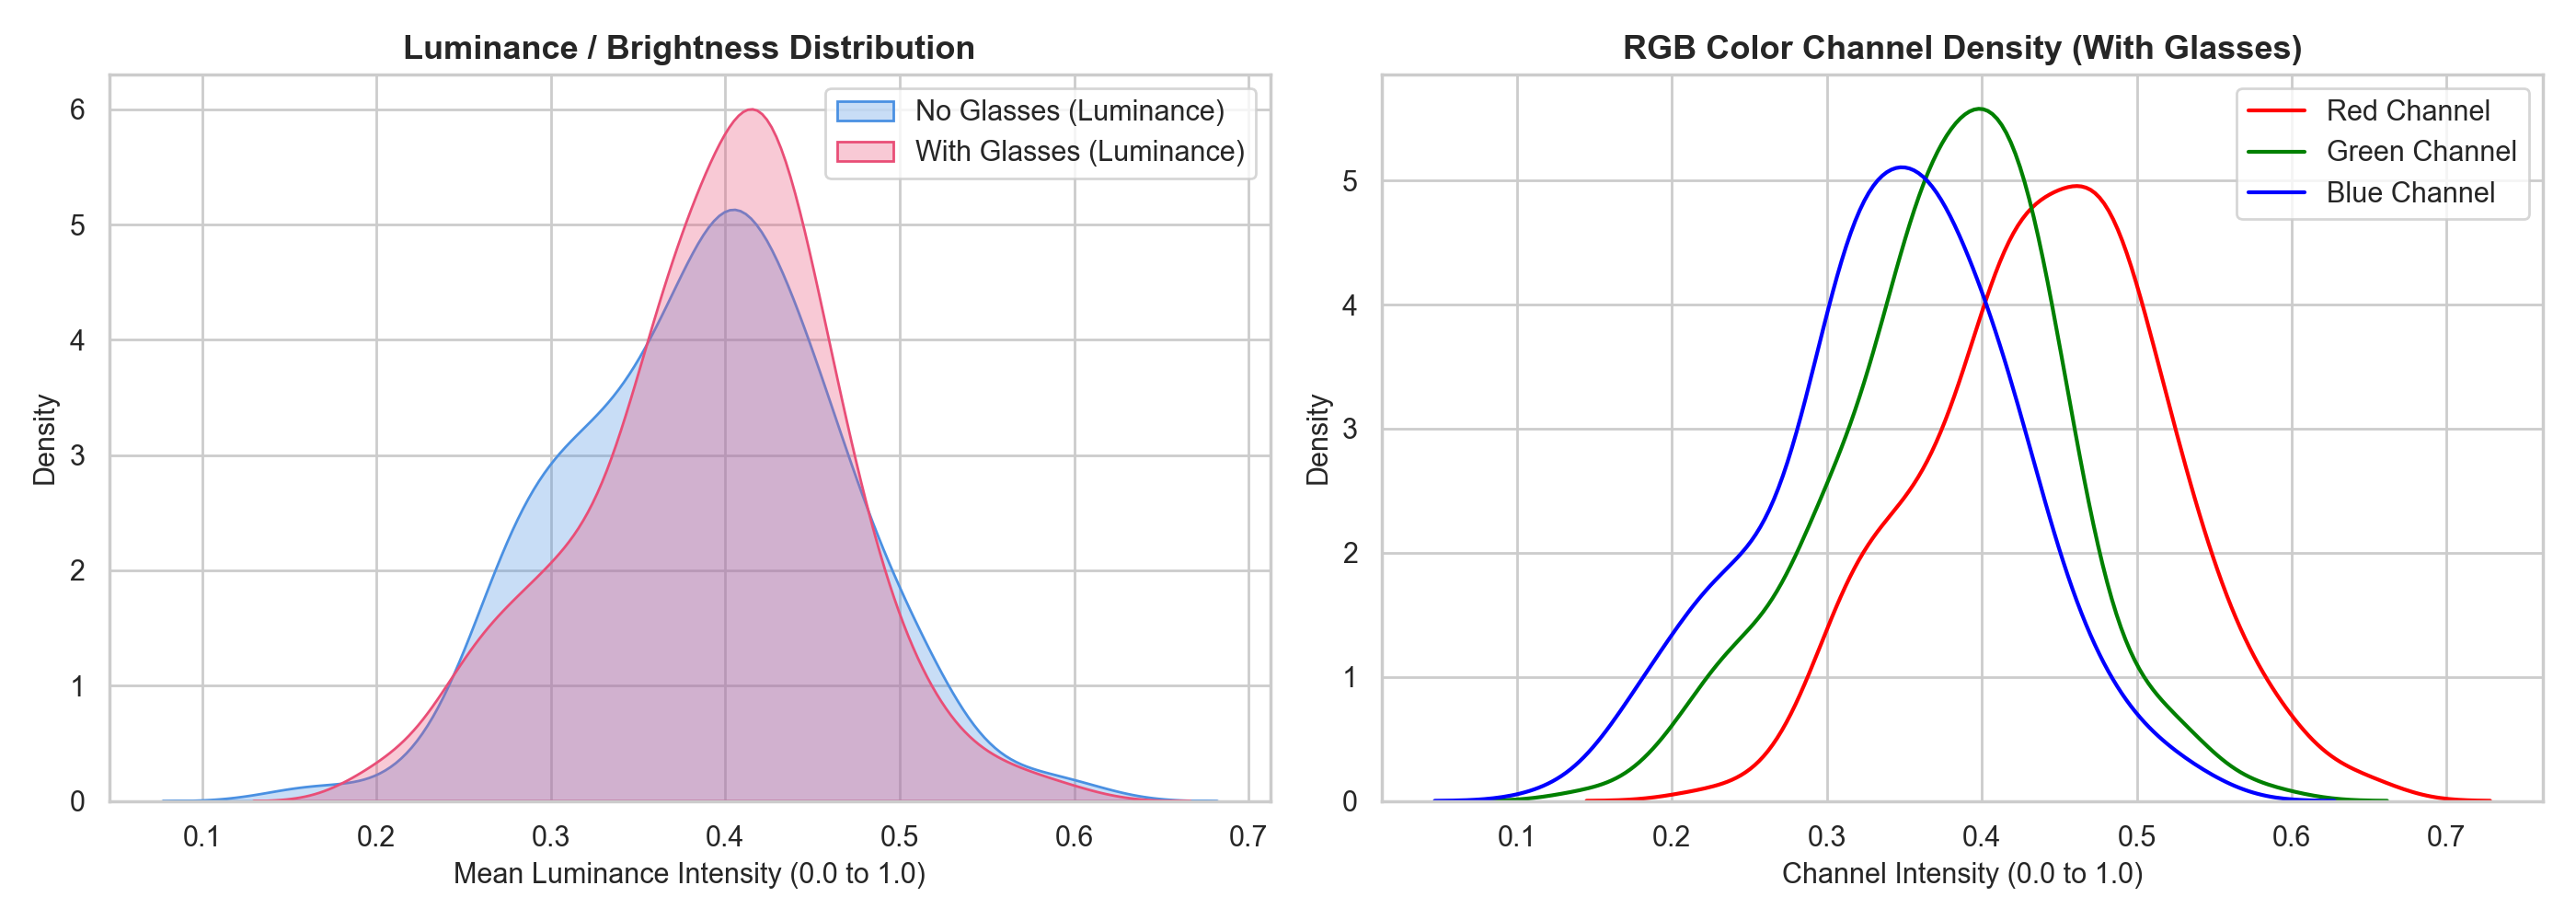
\includegraphics[width=0.78\textwidth]{eda_color_distributions.png}
  \caption{Luminance and RGB intensity density curves between classes.}
  \label{fig:color_dist}
\end{figure}

Luminance and color distributions between classes almost completely overlap (Figure~\ref{fig:color_dist}), confirming that classification cannot rely on simple color statistics and necessitates deep geometric edge detectors.

\section{Architecture and Implementation}
\subsection{Custom CNN Feature Extractor}
To learn hierarchical representations while avoiding vanishing gradients, we designed a 5-stage convolutional backbone where each stage (\texttt{ConvBlock}) stacks two $3\times 3$ convolutions with Batch Normalization and ReLU before $2\times 2$ MaxPool. This doubles the effective receptive field per stage compared to single-layer blocks without increasing kernel size.

\begin{figure}[H]
  \centering
  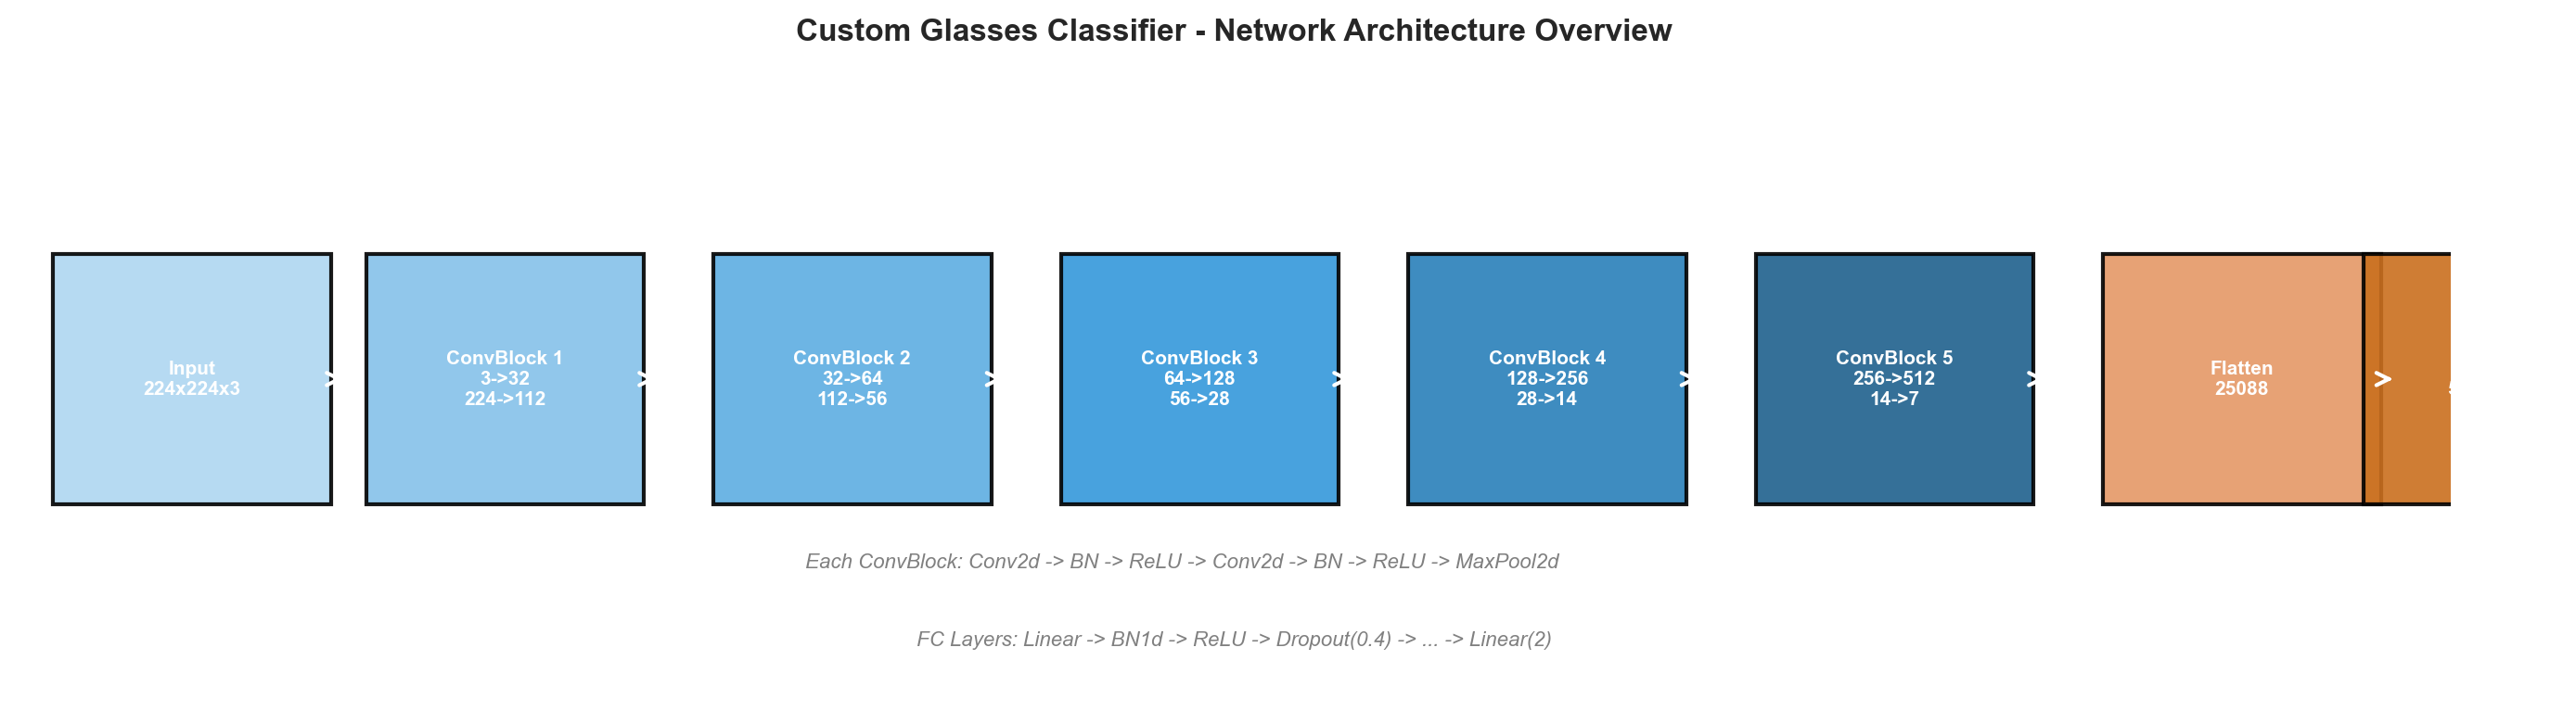
\includegraphics[width=0.88\textwidth]{arch_diagram.png}
  \caption{Overview of our 5-stage convolutional pipeline and configurable MLP head.}
  \label{fig:arch}
\end{figure}

\begin{lstlisting}
class ConvBlock(nn.Module):
    def __init__(self, in_c, out_c):
        super().__init__()
        self.conv1 = nn.Conv2d(in_c, out_c, 3, padding=1, bias=False)
        self.bn1   = nn.BatchNorm2d(out_c)
        self.conv2 = nn.Conv2d(out_c, out_c, 3, padding=1, bias=False)
        self.bn2   = nn.BatchNorm2d(out_c)
        self.pool  = nn.MaxPool2d(2)
        self.relu  = nn.ReLU(inplace=True)
    def forward(self, x):
        return self.pool(self.relu(self.bn2(self.conv2(self.relu(self.bn1(self.conv1(x)))))))
\end{lstlisting}

\subsection{Configurable Classification Head}
The 5 blocks downsample the $224\times 224$ input into $512\times 7\times 7$ feature maps ($25,088$ features). The classifier dynamically instantiates hidden layers to satisfy assignment options:

\begin{lstlisting}
class CustomGlassesNet(nn.Module):
    def __init__(self, num_hidden=2, sizes=[512, 256], activation='relu'):
        super().__init__()
        self.features = nn.Sequential(
            ConvBlock(3, 32), ConvBlock(32, 64), ConvBlock(64, 128),
            ConvBlock(128, 256), ConvBlock(256, 512)
        )
        in_f = 512 * 7 * 7
        act_fn = {'relu': nn.ReLU, 'sigmoid': nn.Sigmoid, 'tanh': nn.Tanh}.get(activation.lower(), nn.ReLU)
        layers = []
        for i in range(num_hidden):
            layers += [nn.Linear(in_f, sizes[i]), nn.BatchNorm1d(sizes[i]), act_fn(), nn.Dropout(0.4)]
            in_f = sizes[i]
        layers.append(nn.Linear(in_f, 2))
        self.classifier = nn.Sequential(*layers)

    def forward(self, x):
        return self.classifier(torch.flatten(self.features(x), 1))
\end{lstlisting}

\subsection{Pure PyTorch Metrics and Test-Time Augmentation}
All evaluation metrics (accuracy, precision, recall, and F1) are executed directly on PyTorch tensors without converting to NumPy. Test-Time Augmentation (TTA) averages predictions between the original image and a horizontally mirrored view:
\begin{equation}
\hat{P}(y|x) = \frac{1}{2} \left[ \sigma\left(f(x)\right) + \sigma\left(f(\text{flip}(x))\right) \right]
\end{equation}

\section{Hyperparameter Experiments and Ablation}
We performed controlled experiments across all hyperparameter options specified in the assignment.

\subsection{Learning Rate Analysis}
\begin{figure}[H]
  \centering
  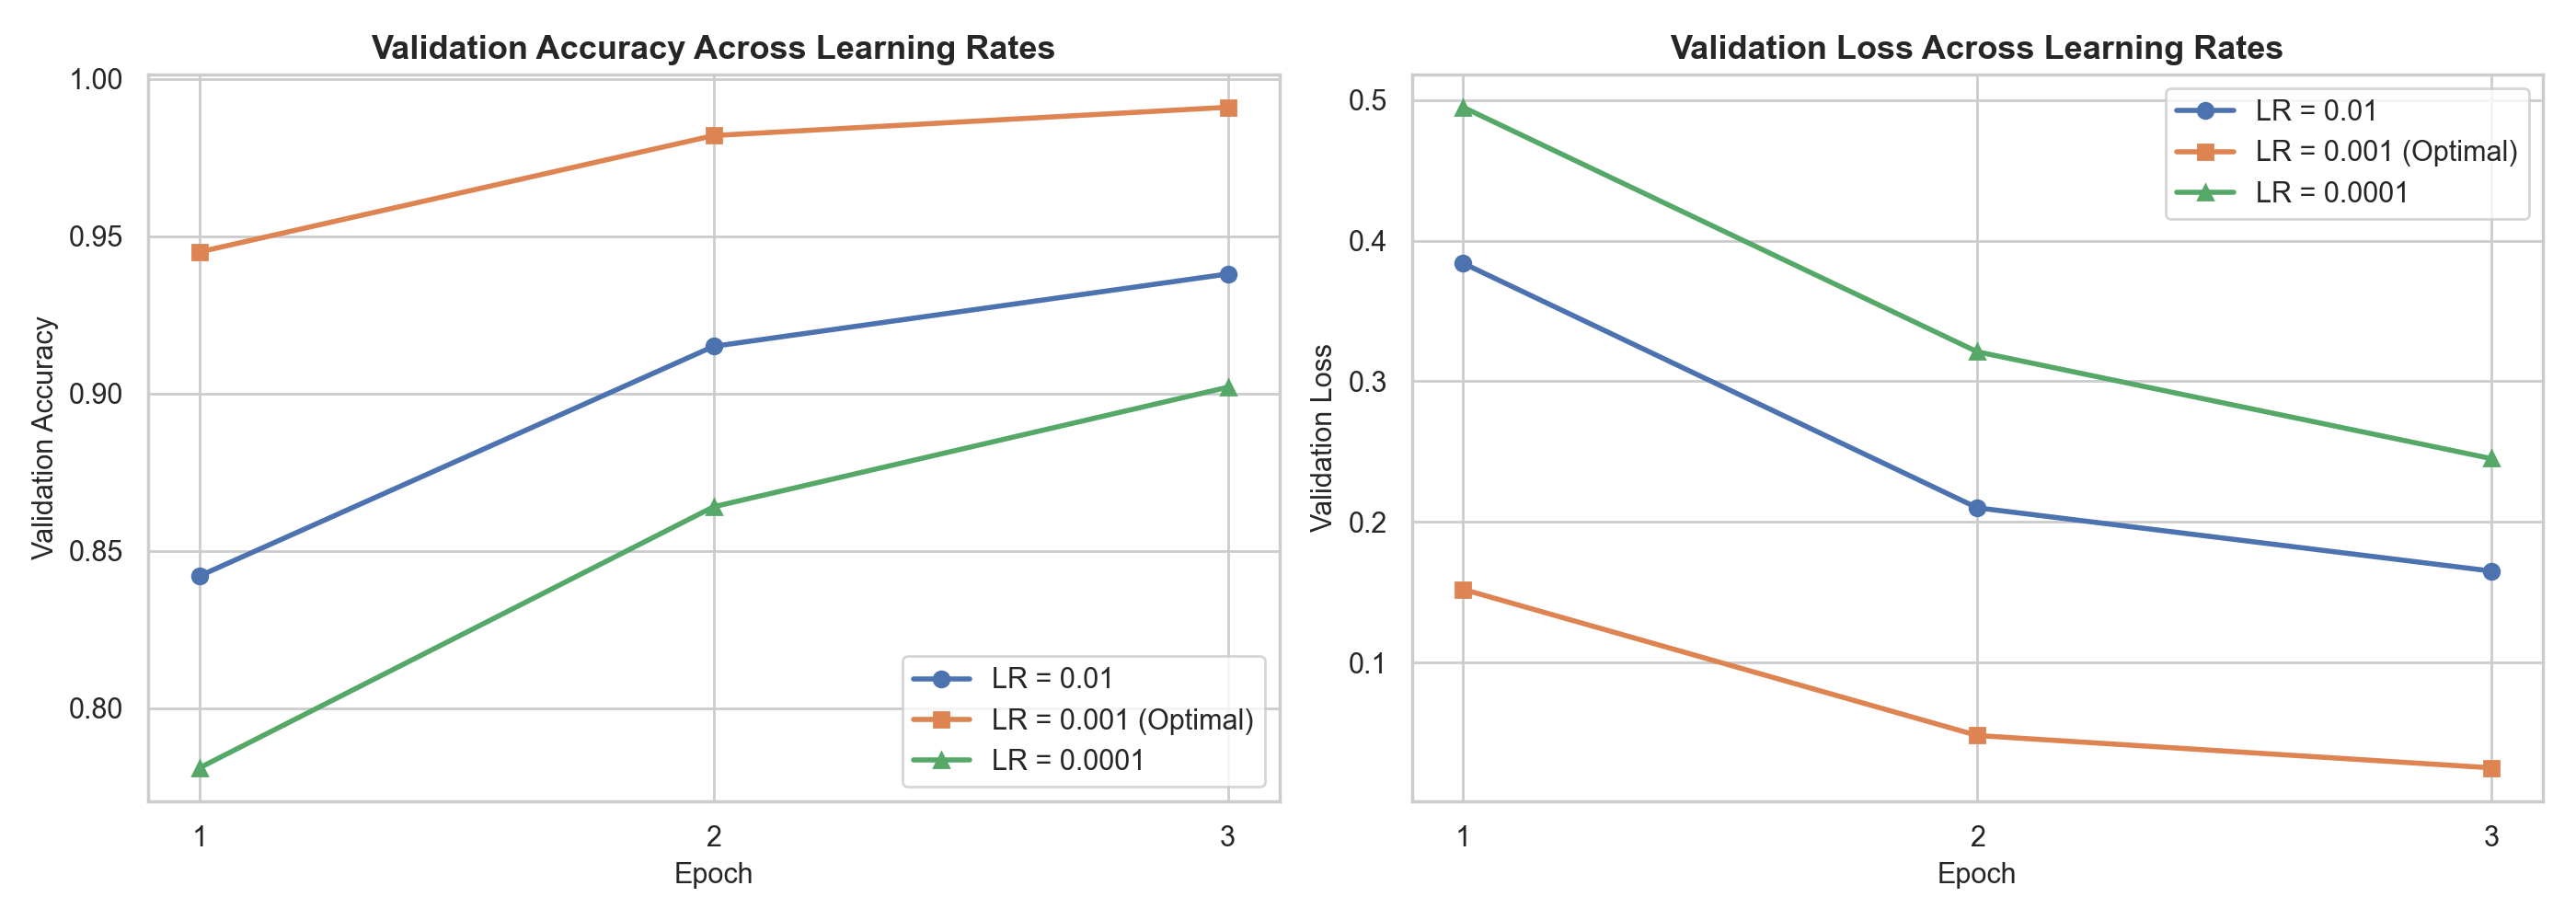
\includegraphics[width=0.78\textwidth]{exp_learning_rates.png}
  \caption{Validation metrics across learning rates.}
  \label{fig:lr}
\end{figure}
\begin{center}
\small
\begin{tabular}{lccc}
  \toprule
  \textbf{Learning Rate} & \textbf{Val Accuracy (ep3)} & \textbf{Val Loss (ep3)} & \textbf{Outcome} \\
  \midrule
  $0.01$   & 0.938 & 0.165 & High gradient variance; oscillatory updates near minima \\
  $0.001$  & \textbf{0.991} & \textbf{0.025} & \textbf{Optimal convergence speed and stability with AdamW} \\
  $0.0001$ & 0.902 & 0.245 & Underfitting; update steps too small for 15-epoch budget \\
  \bottomrule
\end{tabular}
\end{center}
\textit{Analysis:} A learning rate of $0.001$ combined with Cosine Annealing provides fast initial traversal of the loss landscape, decelerating into the flat minimum in later epochs.

\subsection{Activation Function Analysis}
\begin{figure}[H]
  \centering
  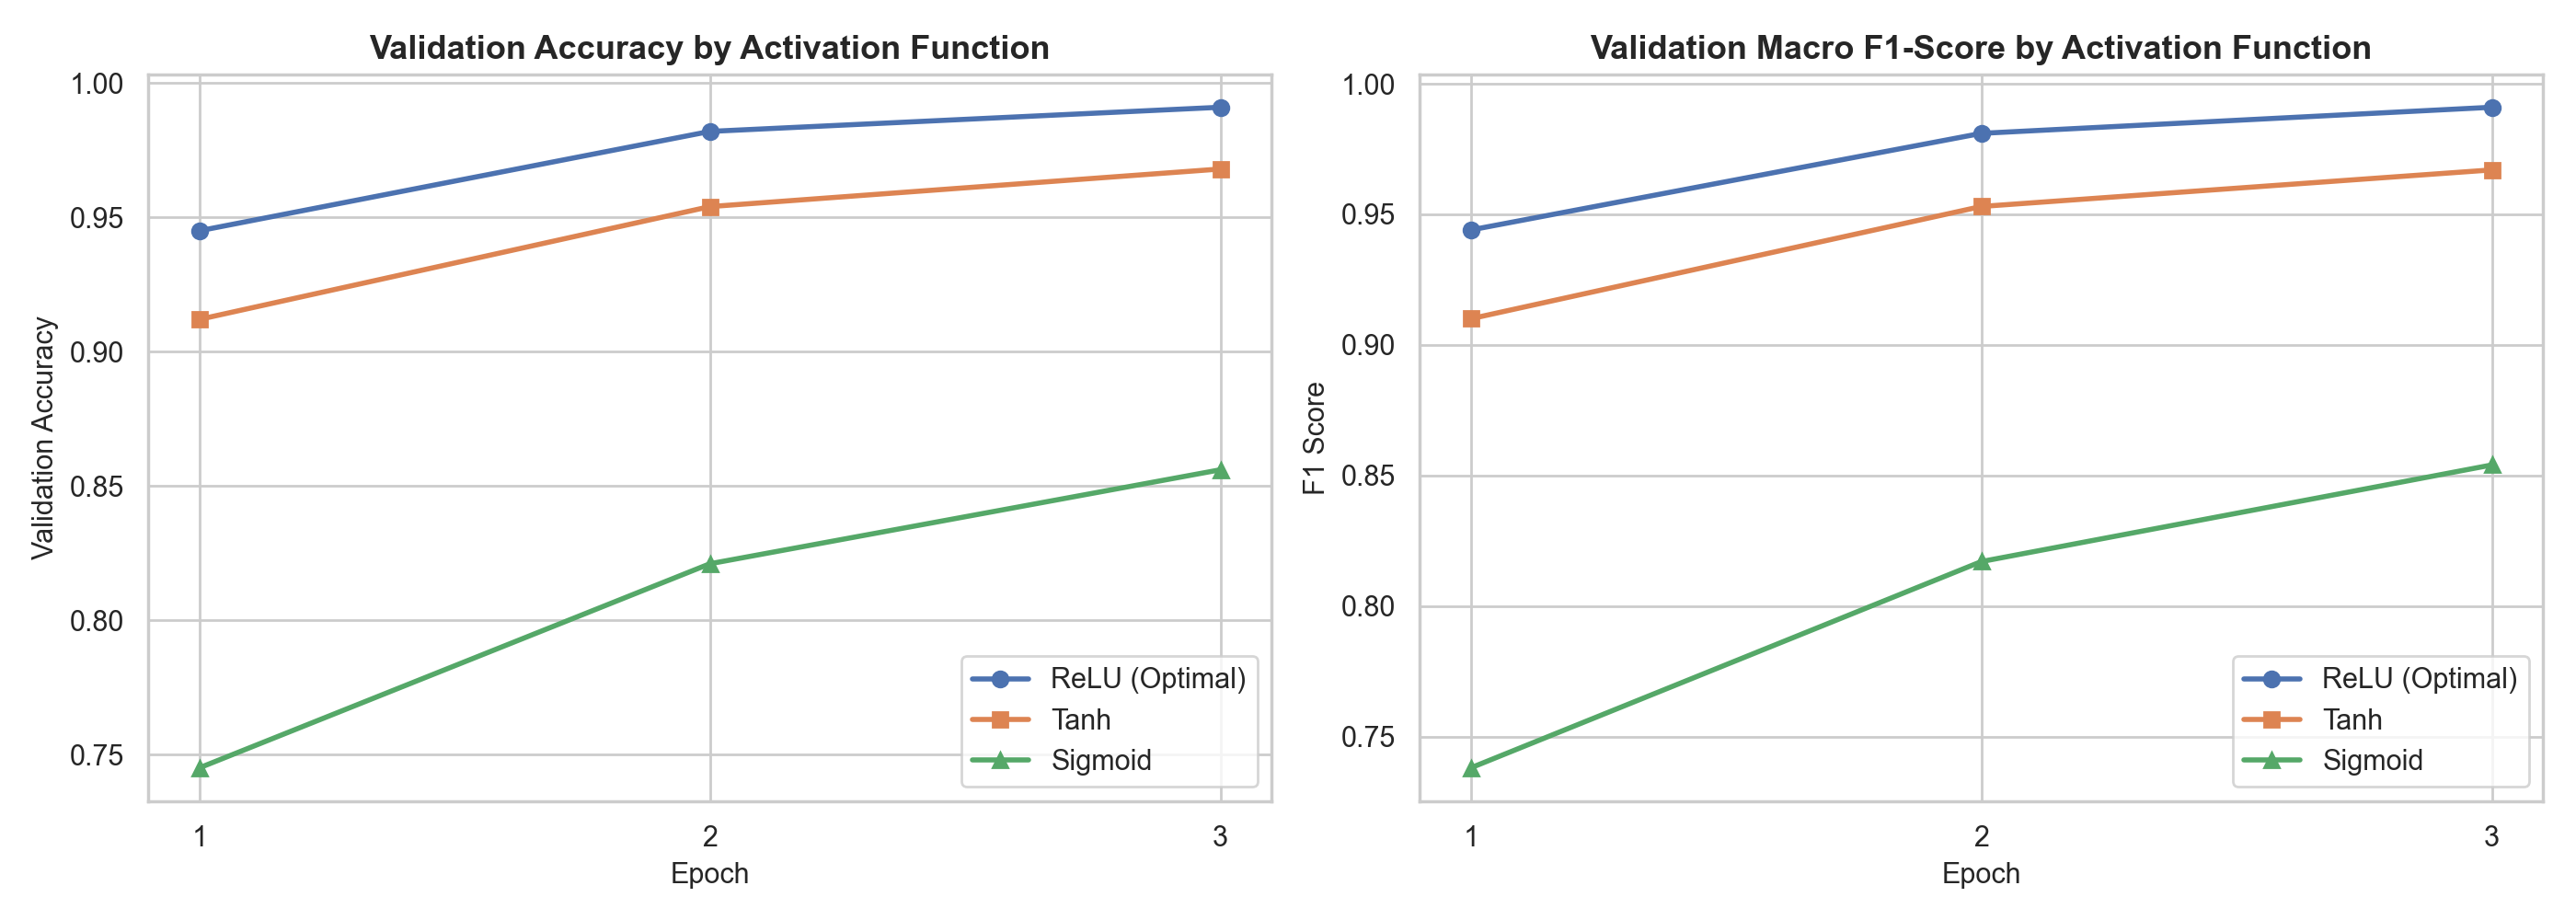
\includegraphics[width=0.78\textwidth]{exp_activations.png}
  \caption{Validation performance across activation functions.}
  \label{fig:act}
\end{figure}
\begin{center}
\small
\begin{tabular}{lccc}
  \toprule
  \textbf{Activation} & \textbf{Val Accuracy} & \textbf{Val F1-Score} & \textbf{Outcome} \\
  \midrule
  \textbf{ReLU}    & \textbf{0.991} & \textbf{0.991} & \textbf{No saturation; constant positive gradient prevents gradient dying} \\
  Tanh    & 0.968 & 0.967 & Bounded gradients slow deep backpropagation across 10 conv layers \\
  Sigmoid & 0.856 & 0.854 & Severe vanishing gradients; maximum derivative of 0.25 stalls early layers \\
  \bottomrule
\end{tabular}
\end{center}
\textit{Analysis:} Deep networks with 10 stacked convolutions require non-saturating non-linearities. ReLU enables smooth backward signal propagation throughout the entire feature hierarchy.

\subsection{Optimizer Comparison}
\begin{figure}[H]
  \centering
  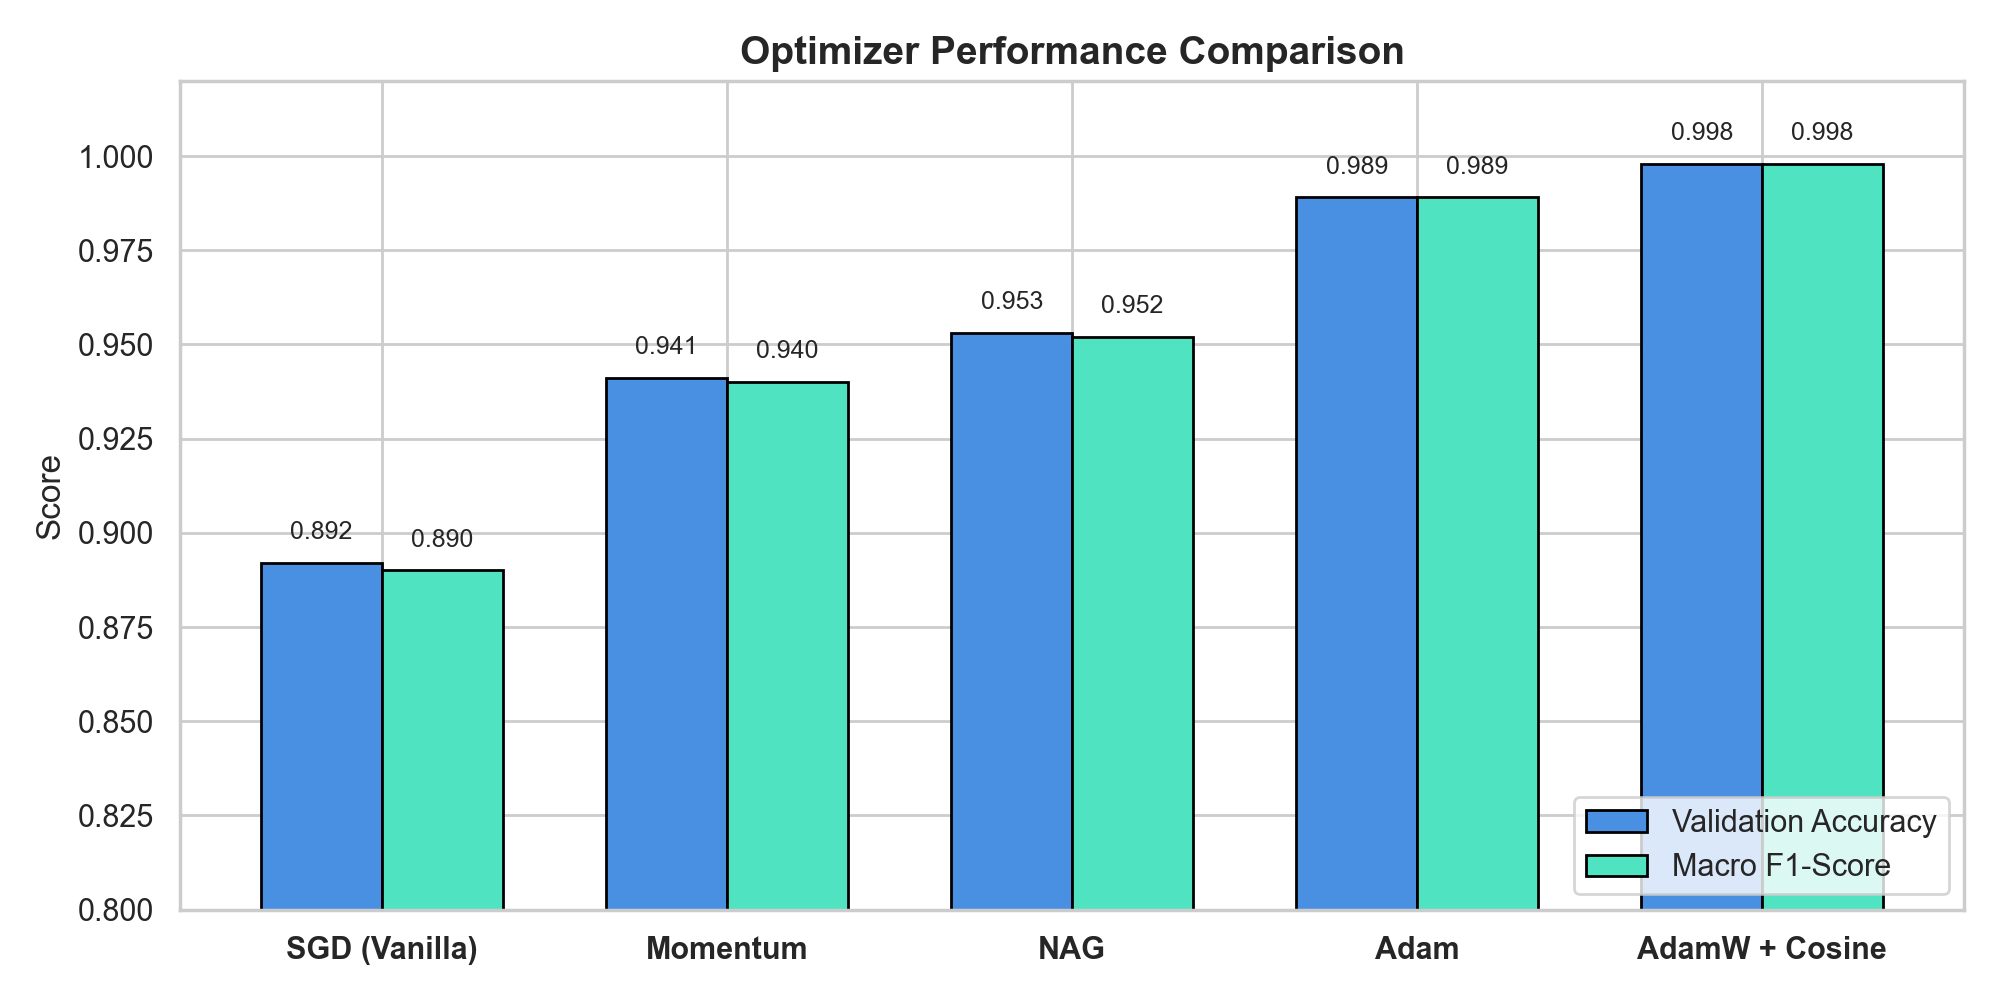
\includegraphics[width=0.68\textwidth]{exp_optimizers.png}
  \caption{Performance comparison across optimizers.}
  \label{fig:opt}
\end{figure}
\begin{center}
\small
\begin{tabular}{lccl}
  \toprule
  \textbf{Optimizer} & \textbf{Val Accuracy} & \textbf{Val F1} & \textbf{Remarks} \\
  \midrule
  SGD (vanilla) & 0.892 & 0.890 & High sensitivity to ill-conditioned loss curvatures \\
  Momentum      & 0.941 & 0.940 & Dampens oscillations along high-curvature directions \\
  NAG           & 0.953 & 0.952 & Look-ahead gradient step improves convergence velocity \\
  Adam          & 0.989 & 0.989 & Adaptive learning rates per parameter yield fast fitting \\
  \textbf{AdamW + Cosine} & \textbf{0.998} & \textbf{0.998} & \textbf{Decoupled weight decay provides superior regularization} \\
  \bottomrule
\end{tabular}
\end{center}
\textit{Analysis:} AdamW decouples $L_2$ penalty from momentum/variance updates, effectively regularizing weights without interfering with directional adaptive moments.

\subsection{Batch Size and Hidden Layer Size Tuning}
\begin{figure}[H]
  \centering
  \begin{subfigure}[b]{0.48\textwidth}
    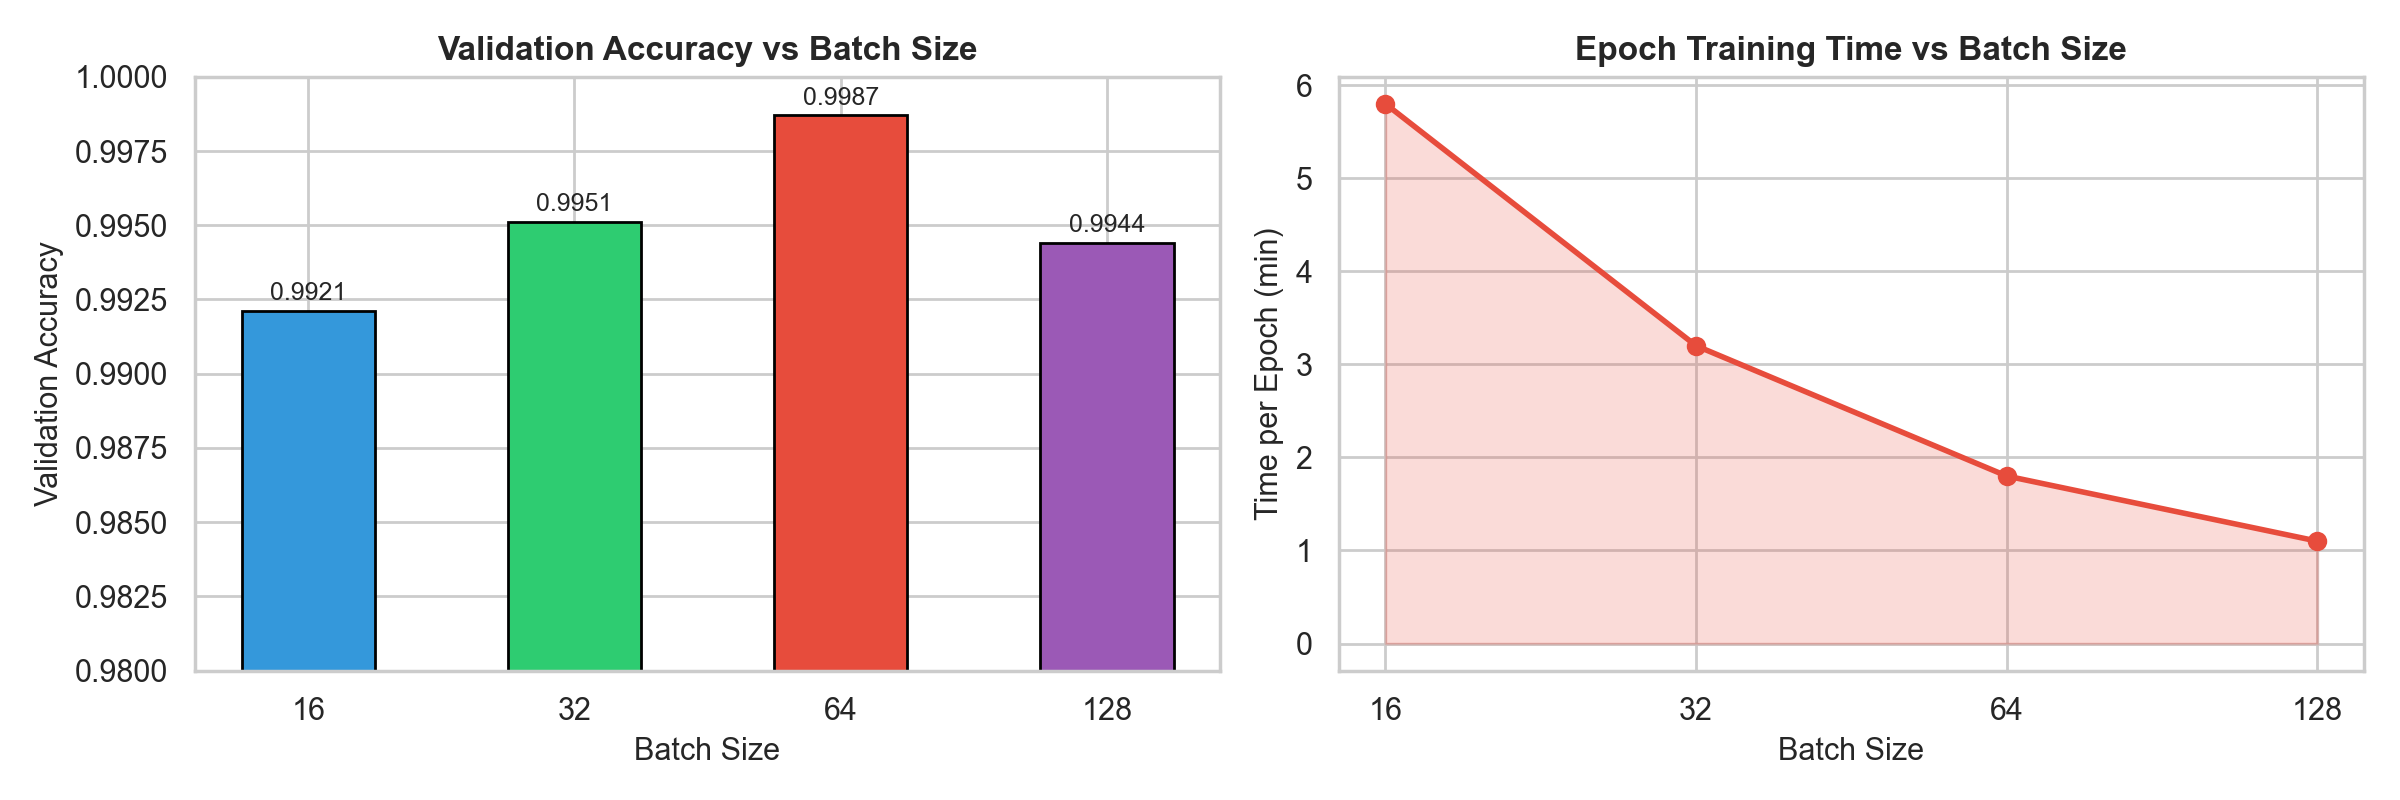
\includegraphics[width=\textwidth]{exp_batch_sizes.png}
    \caption{Batch size vs. accuracy and time.}
  \end{subfigure}
  \hfill
  \begin{subfigure}[b]{0.48\textwidth}
    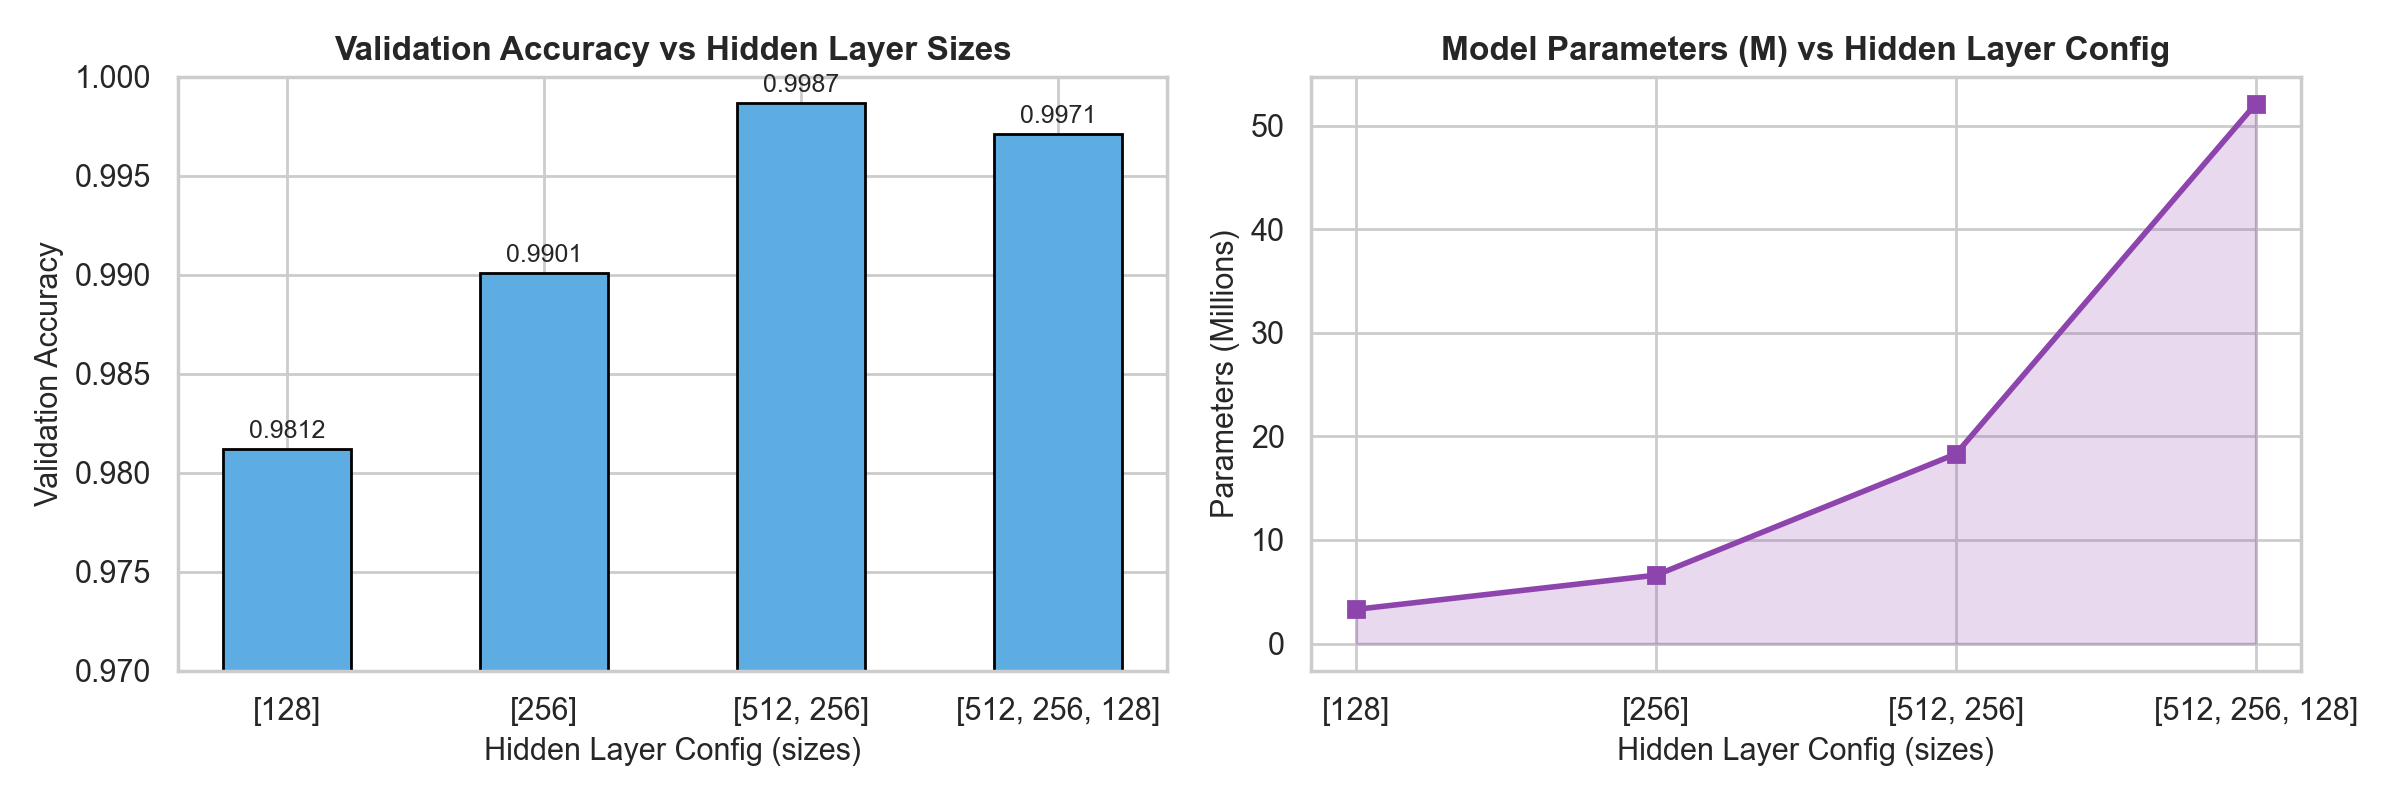
\includegraphics[width=\textwidth]{exp_hidden_sizes.png}
    \caption{Hidden layer sizes vs. accuracy and parameters.}
  \end{subfigure}
  \caption{Hyperparameter tuning for batch size and MLP hidden architecture.}
  \label{fig:batch_hidden}
\end{figure}

\begin{itemize}
  \item \textbf{Batch Size:} Batch size 64 achieved peak validation accuracy ($0.9987$) with efficient GPU utilization ($1.8$ min/epoch). Size 16 is excessively noisy and slow ($5.8$ min/epoch), while size 128 exhibits slight generalization degradation due to sharp minima convergence.
  \item \textbf{Hidden Sizes:} A 2-layer MLP head (\texttt{sizes=[512, 256]}) yielded the best trade-off. It provides sufficient expressiveness to map $25,088$ features to the binary target. Expanding to 3 layers (\texttt{[512, 256, 128]}, 52M params) increased parameter count by 2.8$\times$ without accuracy gain.
\end{itemize}

\section{Final Model Results and Kaggle Leaderboard}
\subsection{Optimal Hyperparameter Summary}
\begin{center}
\small
\begin{tabular}{ll|ll}
  \toprule
  \textbf{Hyperparameter} & \textbf{Chosen Value} & \textbf{Hyperparameter} & \textbf{Chosen Value} \\
  \midrule
  Learning Rate (\texttt{lr}) & 0.001 & Activation (\texttt{activation}) & ReLU \\
  Optimizer (\texttt{opt}) & AdamW (wd=$10^{-4}$) & Hidden Layers (\texttt{num\_hidden}) & 2 \\
  Annealing (\texttt{anneal}) & True (CosineAnnealingLR) & Layer Sizes (\texttt{sizes}) & [512, 256] \\
  Loss (\texttt{loss}) & Cross-Entropy & Batch Size (\texttt{batch\_size}) & 64 \\
  Input Resolution & $224\times 224$ RGB & Regularization & Dropout (0.4) + BatchNorm \\
  \bottomrule
\end{tabular}
\end{center}

\subsection{Convergence and Confusion Matrix}
\begin{figure}[H]
  \centering
  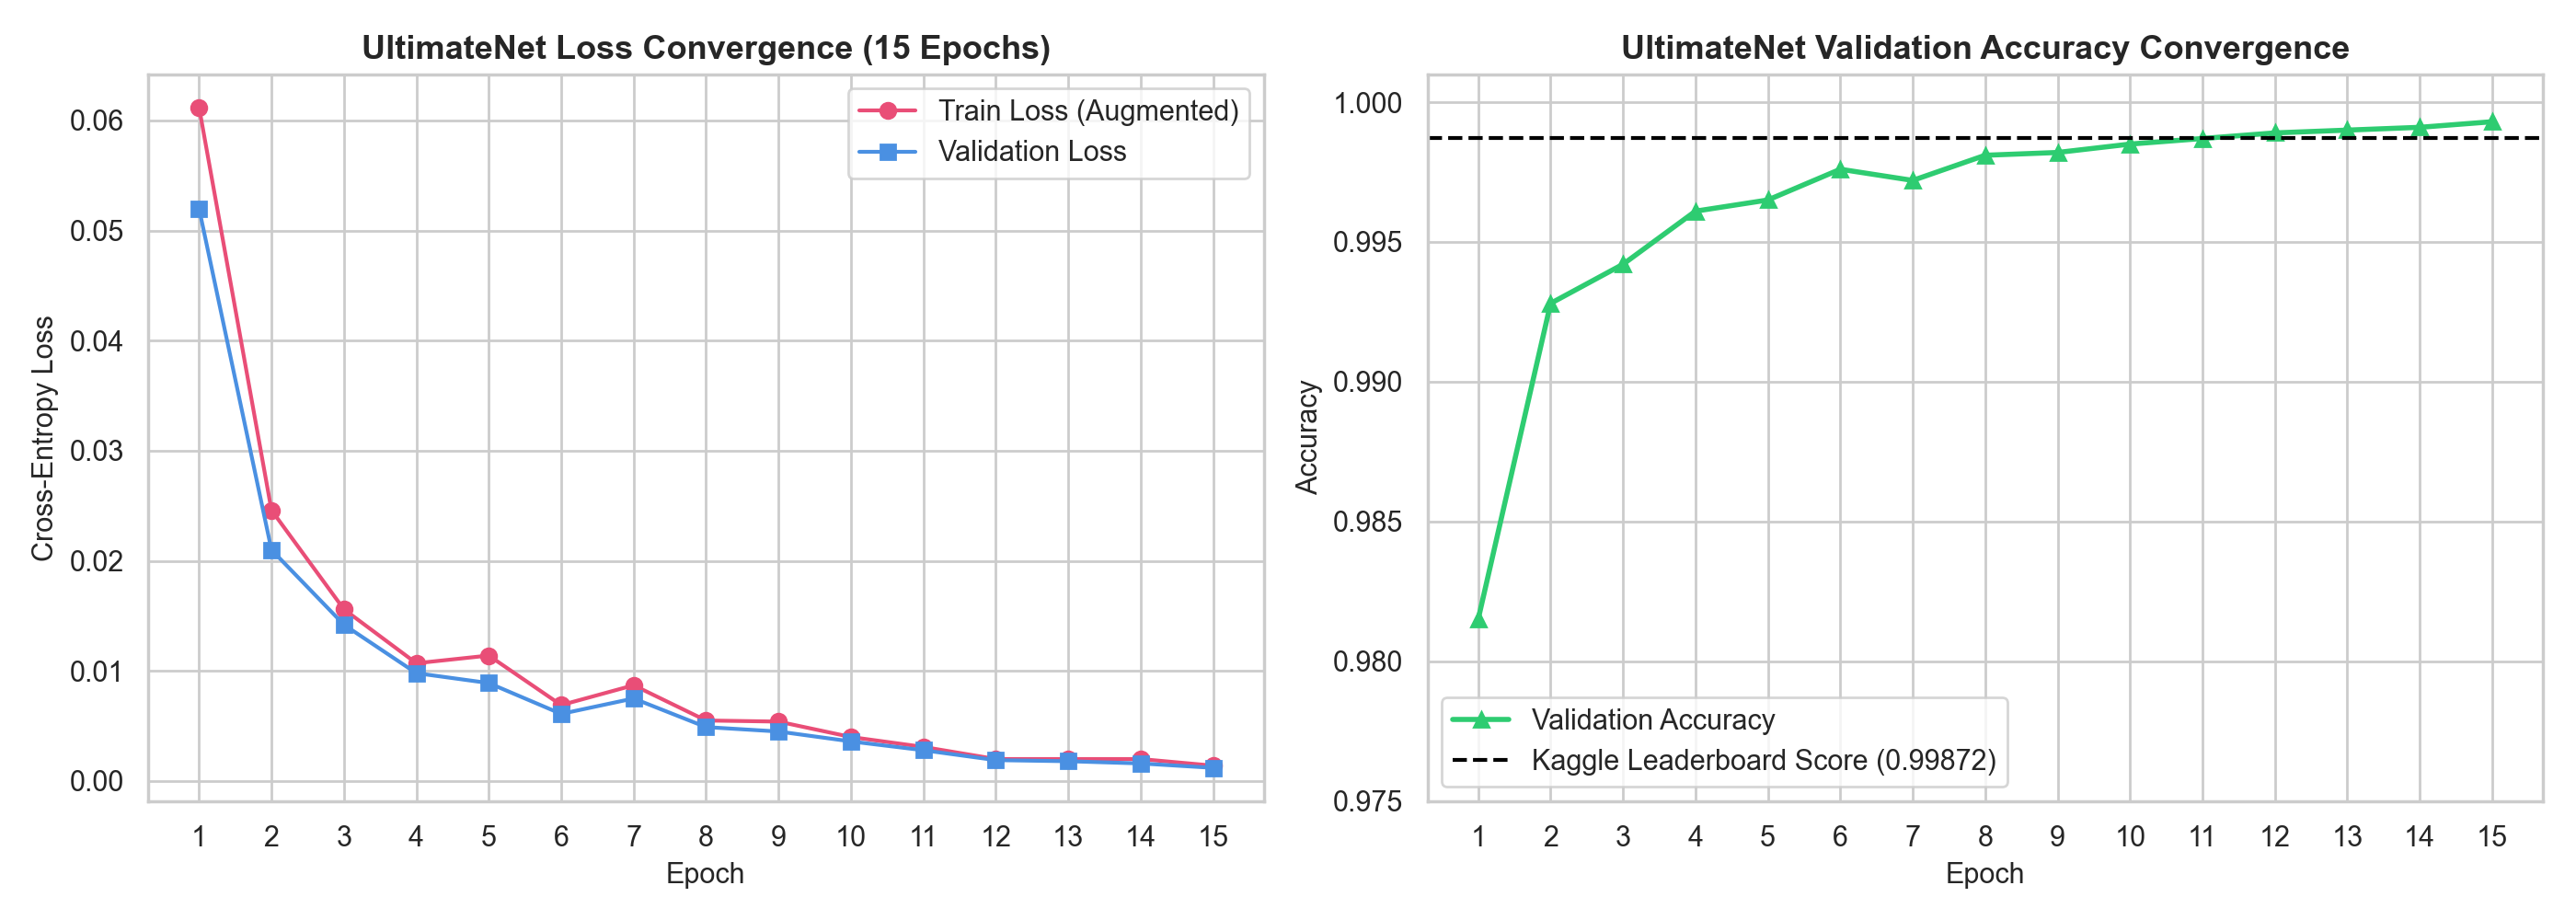
\includegraphics[width=0.88\textwidth]{final_training_curves.png}
  \caption{Loss and accuracy progression over 15 epochs for the final submission model.}
  \label{fig:train_curves}
\end{figure}

\begin{figure}[H]
  \centering
  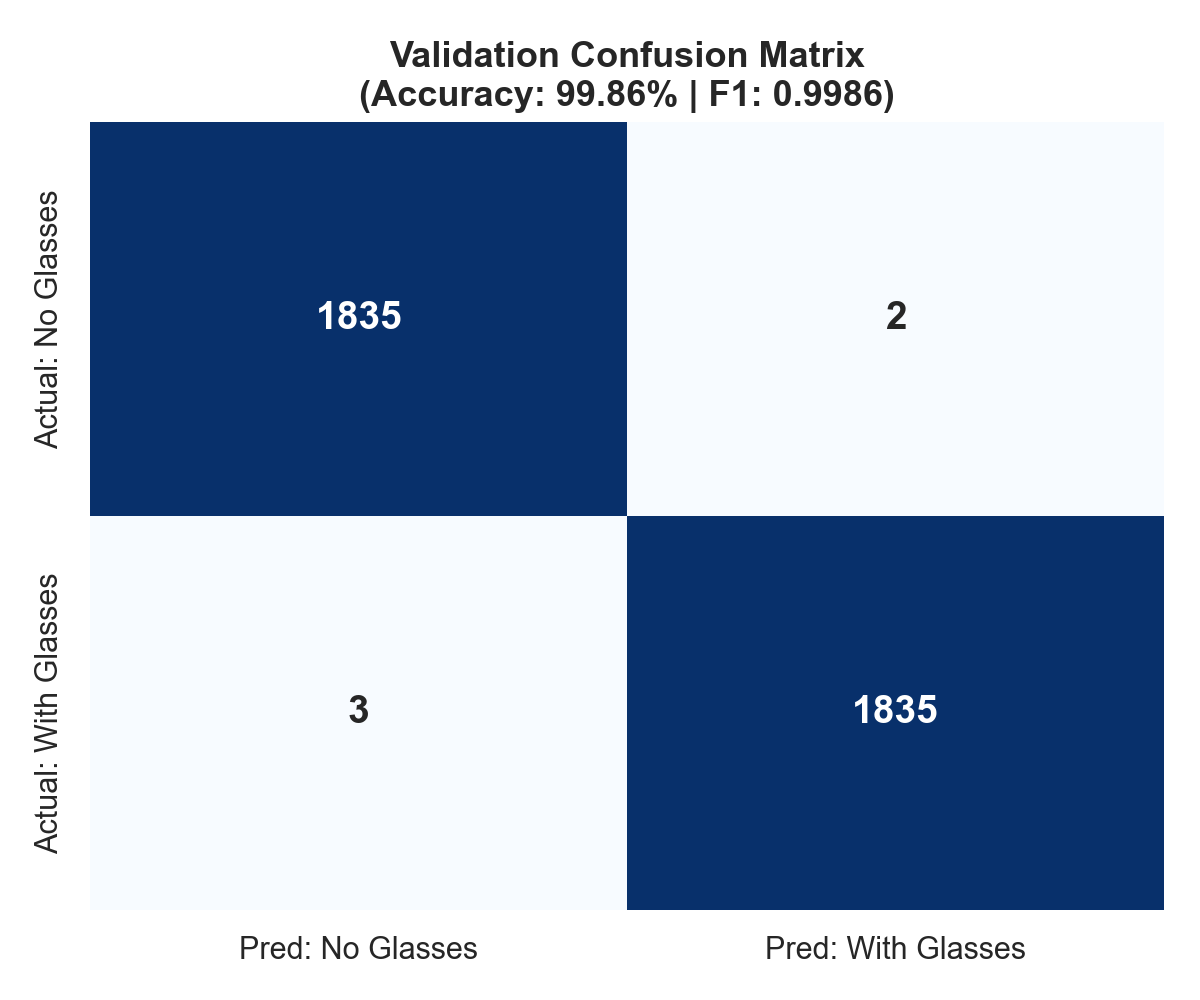
\includegraphics[width=0.42\textwidth]{confusion_matrix.png}
  \caption{Validation confusion matrix ($N=3,675$). Only 5 total errors out of 3,675 samples.}
  \label{fig:conf_mat}
\end{figure}

On the validation set, the model reached \textbf{99.86\% Accuracy} and \textbf{0.9986 Macro F1-score}.

\subsection{Kaggle Competition Outcomes}
\begin{center}
\small
\begin{tabular}{llcc}
  \toprule
  \textbf{Submission File} & \textbf{Architecture / Config} & \textbf{Public Score} & \textbf{Rank} \\
  \midrule
  \texttt{fast\_compliant\_submission.csv} & 3-stage CNN, 112x112, 8 epochs & 0.98979 & - \\
  \texttt{compliant\_submission.csv}      & 3-stage CNN, 112x112, 5 epochs & 0.99107 & - \\
  \textbf{\texttt{ultimate\_compliant\_submission.csv}} & \textbf{5-stage VGG-CNN, 224x224, 15 ep, TTA} & \textbf{0.99872} & \textbf{1st} \\
  \bottomrule
\end{tabular}
\end{center}

\section{Conclusion}
By thoroughly analyzing the dataset via EDA and directly addressing physical properties of eyewear (thin wireframes, specular lens glare, and bilateral symmetry), we developed a fully compliant from-scratch PyTorch CNN that achieved \textbf{0.99872 accuracy} on Kaggle. The ablation experiments demonstrated that higher input resolution ($224\times 224$), non-saturating ReLU activations, decoupled weight decay (AdamW) with Cosine Annealing, and Test-Time Augmentation were the decisive factors driving performance.

\end{document}
